\documentclass[a4paper,11pt]{article}
\usepackage[T2A]{fontenc}     
\usepackage[utf8]{inputenc}  
\usepackage{lmodern}  
\usepackage{amsmath}
\usepackage{amsfonts}
\usepackage{amssymb} 
\usepackage{listings}
\usepackage{lstcustom}
\usepackage{graphicx}
\usepackage{geometry} % Меняем поля страницы
\geometry{left=2cm}% левое поле
\geometry{right=1.5cm}% правое поле
\geometry{top=1cm}% верхнее поле
\geometry{bottom=2cm}% нижнее поле
\renewcommand\lstlistingname{Листинг}
\renewcommand\contentsname{Содержание}
\renewcommand\partname{ }
\renewcommand{\thepart}{\arabic{part}}


 
\author{Архангельский Илья}


\begin{document}
\begin{titlepage}
	\begin{center}
		БЕЛОРУССКИЙ ГОСУДАРСТВЕННЫЙ УНИВЕРСИТЕТ \\
		ФАКУЛЬТЕТ ПРИКЛАДНОЙ МАТЕМАТИКИ И ИНФОРМАТИКИ
	\end{center}
	\vspace{10em}
	\begin{center}
		\LARGE {Лабораторная работа \\
		по вычислительным методам алгебры на тему:}
		\linebreak	 
		
    Нахождение собственных значений и собственных векторов \\
    методом А.Н. Крылова
	\end{center}
	\vspace{3em}
	\begin{flushright}
	  
	
 	Выполнил: \\	Архангельский И.А. \\ 
 	
 	  \vspace{1em}
 	
 	  Проверил: \\ Кондратюк А.П. \\
 	
	\end{flushright}
	
	\vfill
	\begin{center}
		Минск, 2012
	\end{center}
\end{titlepage} 

\newpage
\part*{Входные и выходные данные.} 
\section*{Входные данные}

Входной файл содержит размерность матрицы,  матрицу $A$ и начальный вектор $c_0$
\section*{Выходные данные}
В случае если возможно найти многочлен степени $n$, программа выводит коэффициенты многочлена и ожидает ввода $n$ его корней (собственных значений матрицы $A$).
Далее выполняется расчет и вывод собственных векторов матрицы $A$.
\newpage 
\part*{Блок-схема} 
 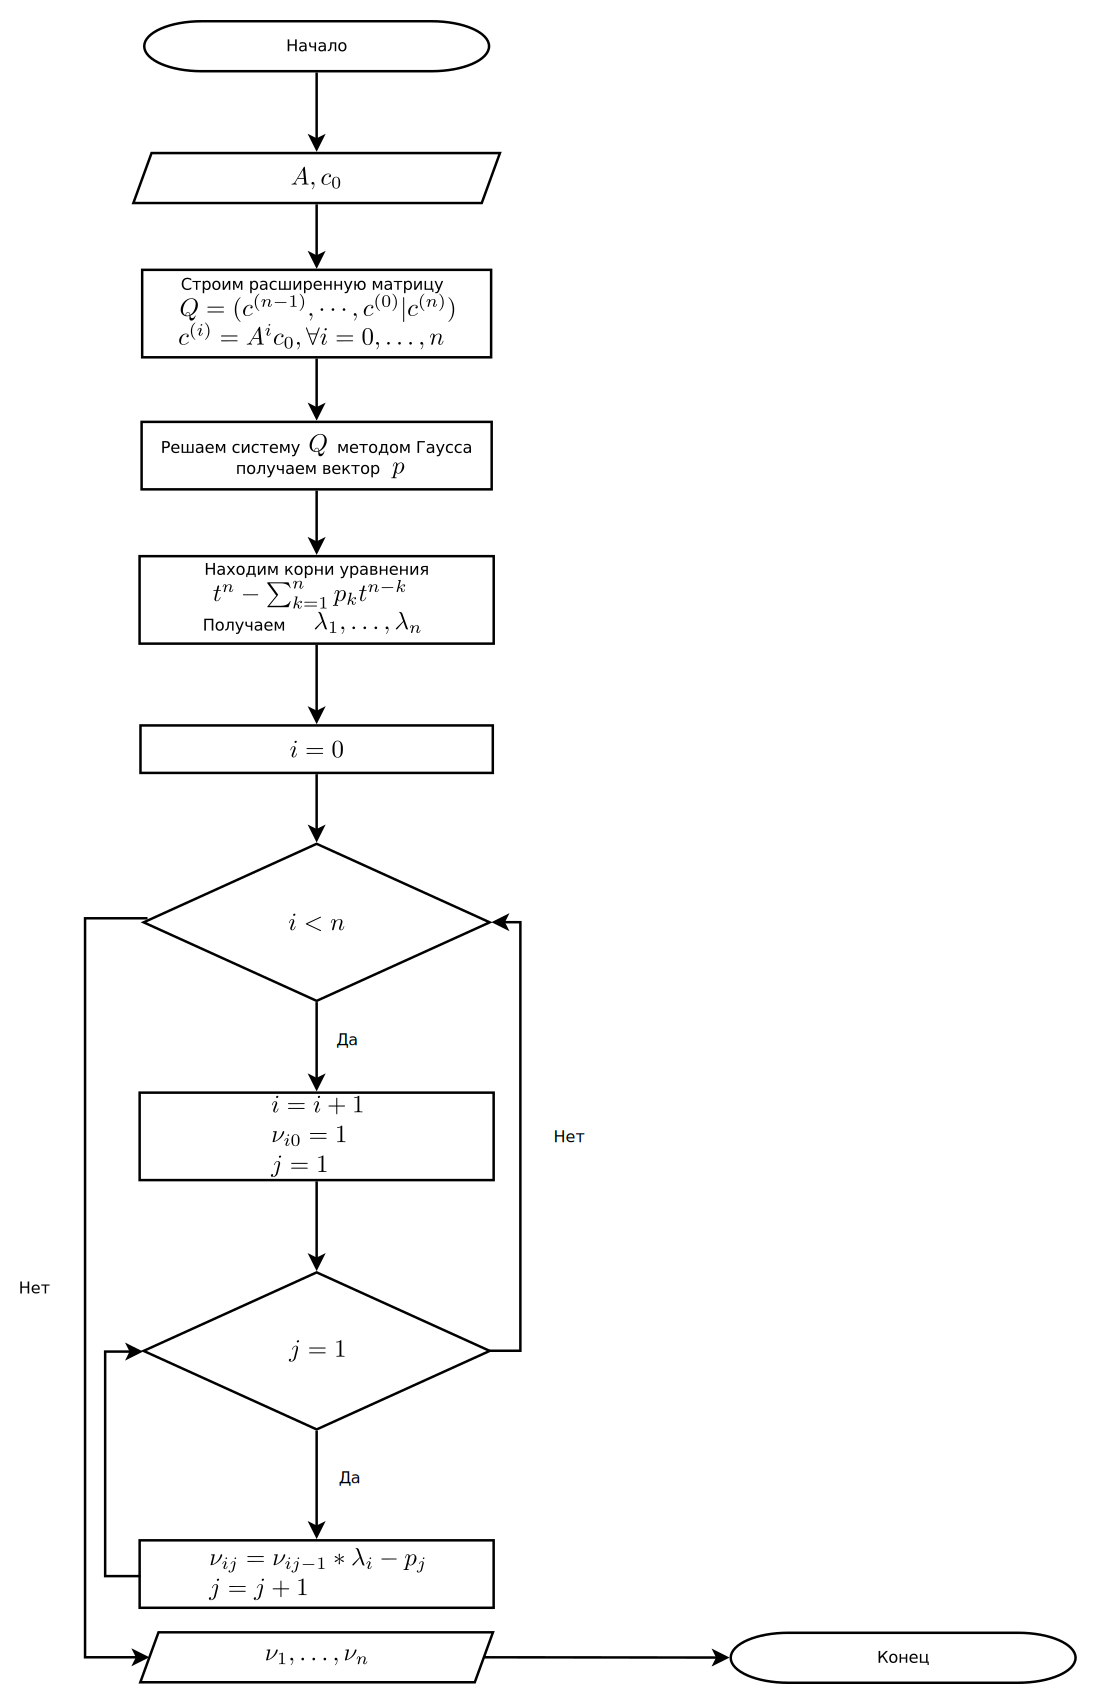
\includegraphics[scale=0.55]{flowchart.pdf} 


\newpage
\part*{Реализация}
\lstinputlisting[language=C++, style=eclipse, basicstyle=\scriptsize, title={krylov.h}]{"../Krylov/krylov.h"}
\lstinputlisting[language=C++, style=eclipse, basicstyle=\scriptsize, title={krylov.cpp}]{"../Krylov/krylov.cpp"}
\lstinputlisting[language=C++, style=eclipse, basicstyle=\scriptsize, title={main.cpp}]{"../Krylov/main.cpp"}
\newpage

 
\newpage
\part*{Тестовые данные}
Матрица:\\ 

$
A=\begin{pmatrix}
-5.509882 &      1.870086&        0.422908&        0.008814\\
0.287865&        -11.811654&      5.711900&       0.058717\\
0.049099&        4.308033&        -12.970687&      0.229326\\
0.006235&        0.269851&        1.397369&        -17.596207\\
\end{pmatrix}
$
 \\
Начальный вектор: 
\[c_0 = (1,0,0,0)\]
Полученный многочлен: 
\[\varphi(t) = t^4 +   47.888430*t^3 +  797.278765*t^2 + 5349.455515*t+12296.550566 \]

Корни многочлена(собственные значения): 
\[\lambda_1 = -17.8633, \lambda_2 = -17.1524, \lambda_3 = -7.5740, \lambda_4 = -5.2987 \]

Собственные вектора, соответсвующие собственным значениям: 
\[\nu_1 = (	1.000,  30.025,  260.931,  688.369  )\]
\[\nu_2 = (	1.000,  30.736,  270.082,  716.900  )\]
\[\nu_3 =(	1.000,  40.314 , 491.937,  1623.523  )\]
\[\nu_4 = (	1.000, 42.590,  571.609,  2320.673  )\]

 
\end{document}
